\documentclass[a4paper,11pt,twocolumn]{article}

\usepackage{lrec2012}

\usepackage{polyglossia}
\setdefaultlanguage[variant=australian]{english}

\usepackage{fontspec}
\usepackage{xunicode}
\usepackage{xltxtra}
\usepackage{natbib}
\usepackage{multirow}
%\usepackage{fullpage}
\usepackage{multirow}
\usepackage[colorlinks=true,citecolor=black,linkcolor=black,urlcolor=blue]{hyperref}

\usepackage{booktabs}
\usepackage{jnwmaps}

\defaultfontfeatures{Mapping=tex-text}
\setromanfont{Times New Roman}
\newfontfamily\symbl[Scale=MatchLowercase]{FreeSerif}

\newcommand{\tags}[1]{\texttt{#1}}

\bibdata{kipchak-paper}


\title{Finite-state morphological transducers for three Kypchak languages}

\author{Jonathan North Washington \\
Departments of Linguistics and Central Eurasian Studies\\
Indiana University\\
Bloomington, IN 47405 (USA)\\
\texttt{jonwashi@indiana.edu} \and
Ilnar Salimzyanov  \\
Kazan Federal University \\
Kazan, Republic of Tatarstan\\
(Russian Federation) \\
\texttt{ilnar.salimzyan@gmail.com} \and 
Francis M. Tyers\\
Departament de Llenguatges i Sistemes Informàtics \\  
Universitat d'Alacant\\
E-03071 Alacant (Spain)\\
\texttt{ftyers@dlsi.ua.es} 
}

%FIXME: usually star comes first, then daggers
\name{Jonathan North Washington$^\dagger$, Ilnar Salimzyanov$^\ddagger$, Francis M. Tyers$^\star$}

\address{$^\dagger$Departments of Linguistics and Central Eurasian Studies\\
Indiana University\\
Bloomington, IN 47405 (USA)\\
\texttt{jonwashi@indiana.edu} \and
$^\ddagger$Institut für Maschinelle Sprachverarbeitung \\
Universität Stuttgart\\
Stuttgart (Germany) \\
\texttt{ilnar@ilnar} \and 
$^\star$Departament de Llenguatges i Sistemes Informàtics \\  
Universitat d'Alacant\\
E-03071 Alacant (Spain)\\
\texttt{ftyers@dlsi.ua.es} 
}

\abstract{This paper describes the development of free/open-source finite-state morphological transducers for three Turkic languages---Kazakh, Tatar, and Kumyk---representing a language from each of the three subbranches of the Kypchak branch of Turkic.  The finite-state toolkit used for the work is the Helsinki Finite-State Toolkit (HFST).  This paper describes how the development of a transducer for each subsequent language took less time.  An evaluation is presented which shows that the transducers all have production-level coverage---around 90\%---on freely available corpora of the languages, and high precision and recall over a manually verified test set. \\
	\Keywords{Kazakh, Tatar, Kumyk, morphology, transducer}
}

\begin{document}

\maketitleabstract{}

\section{Introduction}

This paper describes the development of morphological transducers for three closly related languages: Kazakh, Tatar, and Kumyk.

%FIXME: brief background on how, when, and with what support were developed?
The transducers for these languages 

% FIXME: what are transducers used for ?

\section{Languages}

The three languages for which transducers were developed belong to the Northwestern branch of Turkic, which is often referred to as the Kypchak branch.  This branch can be divided into three subbranches.  Kumyk is a member of the Western Kypchak group, Tatar is a member of the Northern Kypchak group, and Kazakh is a member of the Southern Kypchak group \citep[82-83]{histofturkic}.  As such, each of these three languages represents a different one of the three branches of Kypchak.  The geographic distribution of the languages is shown in map \ref{map1}.

\begin{map*}[htbp]
	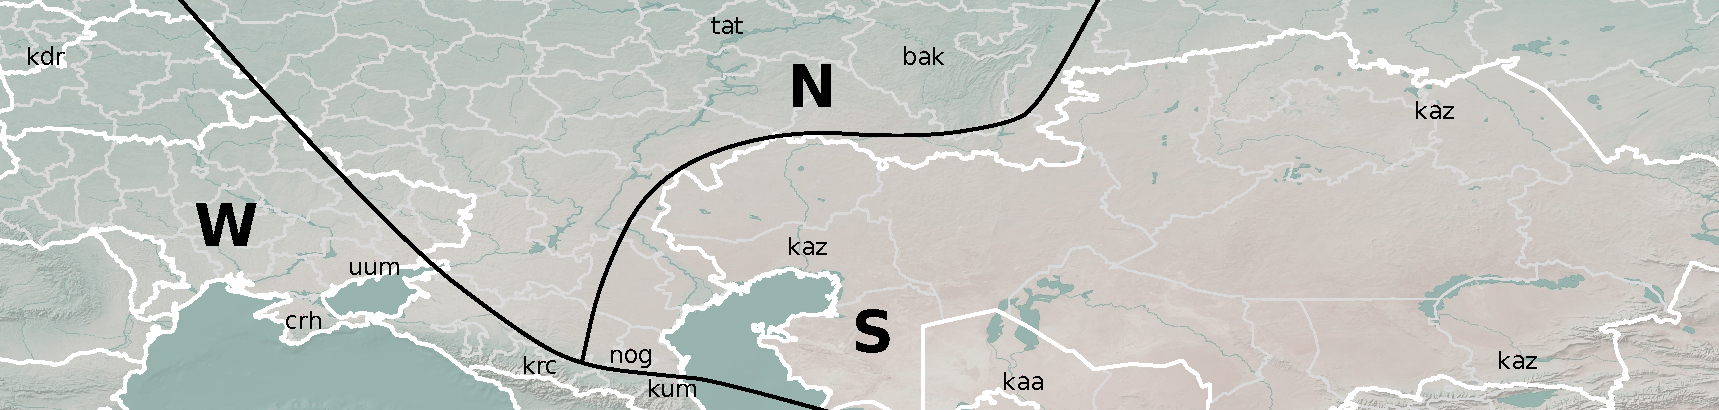
\includegraphics[width=\textwidth]{map/map}
	\caption{The three sub-branches of Kypchak (North, South, West), roughly divided with black lines, showing the geographic distribution of the three languages for which transducers were developed (\texttt{tat}, \texttt{kaz}, \texttt{kum}).  Language codes are from ISO 639-3.}
	\label{map1}
\end{map*}

These languages have different amounts of linguistic influence from other Turkic branches (e.g., moderate Oghuz (SE) influence in the Western group, slight Oghuz influence in the Northern group) and from Mongolic languages (moderate influence on the Southern group, lighter in the other groups), and all have heavy influence from Persian.

\subsection{Kazakh}
Kazakh /q{\symbl ɑ}z{\symbl ɑ}q/ is spoken primarily in Kazakhstan, where it is the national language, sharing official status with Russian as an official language.  Large communities of native speakers also exist in China, neighbouring Central-Eurasian republics, and Mongolia.  Estimates of the total number of speakers range from 8 million \citep{ethnologue} to 11 million \citep{nationalencyklopedin} people.

\subsection{Tatar}
Tatar /t{\symbl ɒ}t{\symbl ɑ}r/ is spoken in and around Tatarstan by approximately 5.4 million people \citep{ethnologue}.  It is co-official with Russian in Tatarstan --- a republic within Russia.  A majority of native speakers of both languages are bilingual in Russian. %, and the standard varieties our system FIXMEs are written in Cyrillic.

\subsection{Kumyk}
Kumyk /qumuq/ is spoken in Dagestan, a Republic of the Russian Federation, where it is co-official with a number of other languages of Dagestan \citep{ethnologue}.  There are approximately 430 thousand speakers \citep{ethnologue}.

\section{Background}
\subsection{Morphological transducers, previous work}
%FIXME: need a source, maybe something by Tommi?
The objective of a morphological transducer is twofold: firstly to take surface forms (e.g., алдым) and generate all possible lexical forms, and secondly to take lexical forms (e.g.,  ал{\tt {\small <v><tv><ifi><p1><sg>}}, алд{\tt {\small <n><px1sg><nom>}}, etc.) and generate one or more surface forms.  Since they are implemented as finite-state automata, they are reversible by default.

The transducers were designed based on the Helsinki Finite State Toolkit \citep{hfst/2011} which is a free/open-source reimplementation of the Xerox finite-state toolchain, popular in the field of morphological analysis.  It implements both the \textbf{lexc} formalism for defining lexicons, and the \textbf{twol} and \textbf{xfst} formalisms for modeling morphophonological rules.  It also supports other finite state transducer formalisms such as \textbf{sfst}.  This toolkit has been chosen as it -- or the equivalent XFST -- has been widely used for other Turkic languages, such as Turkish \citep{coltekin2010}, Crimean~Tatar~\citep{altintas2001}, Turkmen \citep{tantug2006}, and Kyrgyz \citep{washington2012}, and is available under a free/open-source licence.

The authors learned of another Kazakh morphological transducer in existence \citep{bekmanova2013} only after production-ready version of our transducer was released.  We have not yet been able to evaluate this system or compare it to ours.

Creating a morphological transducers in the above-mentioned formalisms simply involves encoding linguistic knowledge about the language in the formalisms.  The lexc and twol formalisms resemble linguistic formalisms, allowing the coders to work with abstractions resembling linguistic categories such lexemes, morphemes, phonemes, and even archiphonemes---as opposed to a raw FST, where input characters are translated to output characters along a graph.

\subsection{Description}

%FIXME: keep revision number up to date
The transducers are available / under development in apertium's subversion repository,\footnote{\url{https://svn.code.sf.net/p/apertium/svn/languages/}} in the directories apertium-kaz, apertium-tat, and apertium-kum.  The revision of the entire subversion repository that the numbers (stem counts, evaluation, etc.) in this paper represent is \texttt{r48137}.


\section{Methodology}
% cite Hengeveld (1992) ?

% Noun morphotactics -- is basically equivalent in all three, except for archiphonemes
% Adjective categorisation
% Adverb categorisation
% "Irregular" harmony, caused by orthography
% Non-finite verb form categorisation "converbs"

% Handling numerals and acronyms.

% Russian loans not obeying phonology N5, e.g. ё vs . самолёт


\subsection{Development effort}

The three transducers discussed in this paper are for Kazakh, Tatar, and Kumyk.  The Kazakh and Tatar transducers were originally created as part of an experimental Kazakh-Tatar machine translation system in December of 2010.  The Kazakh transducer was expanded during Google Code-In 2010 and 2011, and the Tatar transducer was expanded as part of a prototype Tatar and Bashkir machine translation system \citep{tyerswashingtonsalimzyanbattalov12}.  The Kazakh-Tatar machine translation system, along with the two transducers, was expanded to production-level quality as part of a Google Summer of Code project in 2012 \citep{salimzyanov2013}.

The Kumyk transducer was developed starting at the beginning of October, 2013 as experiment to see how difficult it would be to extend lessons learned from the development of the Tatar and Kazakh transducers to a related language.  While the Kazakh and Tatar transducers took years of part-time work to reach their current production-quality (around 90\%) coverage of corpora, the Kumyk transducer only took a couple weeks to reach this level of quality.  This paper explores how the development of the Kumyk transducer benefited from knowledge gained from the development of the Tatar and Kazakh transducers.

The morphotactics of Turkic languages are complex enough that even a linguist who is fluent in the language and has a good linguistic understanding of it may not understand how exactly all morphemes combine.  Native speakers educated about the morphology of their languages also do not have an explicit knowledge of the complete morphotactics.  Hence it often becomes necessary to use fieldwork methodology to elicit the full extent of the morphotactics, be this a linguist with no to little knowledge of a Turkic language working with a native speaker, or a native speaker who understands the extent of what knowledge is necessary to encode in the transducer.  When there is no native speaker of a particular language available, the authors have found that information previously encoded about a closely related language or the intuitions of a speaker of a closely related language may be combined with the use of textual corpora to ``elicit'' information about the morphotactics of a language.  Depending on the contents of corpus and chance, this may not result in a completely accurate model, but it is possible to be thorough.

The Kazakh morphotactics were originally developed based on the Kyrgyz transducer, which was co-authored by a linguist who is fluent in and has a good linguistic knowledge of Kyrgyz together with a native speaker of Kyrgyz, and in consultation with another native speaker of Kyrgyz.  The initial developer of the Kazakh morphotactic was the same linguist, who is fluent in and has a good linguistic understanding Kazakh.  The morphotactics of Tatar were developed for the most part by a native Tatar speaker, who also worked to polish off the morphotactics of the Kazakh transducer.

As the authors found it difficult to locate native speakers of Kumyk, the morphotactics of the Kumyk transducer were developed based on the existing encoded morphotactics of Kazakh and Tatar (and occasionally Kyrgyz), with consultation of corpora, as described above.  A dictionary \citep{bammatov1960} and a grammar \citep{olmesov2000} of Kumyk were also consulted as needed.

% FIXME: how long it took
% FIXME: make a graph for the kumyk one

\subsection{Transducer contents}

Each transducer's lexc source consists of lists of stems, with each stem pointing at a complex continuation lexicon containing the appropriate morphology for the type of stem.  

%FIXME: update for the three languages
The tagset for each transducer is designed to be compatible with the others.  Each transducer consists of about 120 separate tags, of which close to 20 cover the main parts of speech (noun, verb, adjective, adverb, postposition, interjection, etc.).  The remaining tags cover morphological subcategorisation for e.g.\ case, number, person, possession, transitivity, tense-aspect-mood, etc.  The tags are represented as multicharacter symbols, between less-than \texttt{<} and greater-than \texttt{>} symbols.  The tagset is quite extensive and still not entirely stabilised, so a full listing is not included here.  However, the tags are listed in the source code of the transducers, along with comments describing their usage.

%\subsection{Statistics}

Table \ref{table:stems} lists the number of stems of the primary categories in each transducer.

\begin{table}
\begin{center}
\begin{tabular}{lrrr}
		\toprule
\multirow{2}{*}{\textbf{Part of speech}} & \multicolumn{3}{c}{\textbf{Number of stems}} \\ \cline{2-4}
                        & Kazakh & Tatar & Kumyk \\
		\midrule
		Noun & 2463 & 2692 & 2588 \\
		Verb & 1587 & 1333 & 262 \\
		Adjective & 823 & 852 & 217 \\
		Proper noun & 5412 & 3523 & 1444 \\
		Adverb & 197 & 205 & 63 \\
		Numeral & 63 & 67 & 45 \\
		Conjunction & 52 & 50 & 15 \\
		Postposition & 56 & 46 & 12 \\
		Pronoun & 17 & 17 & 18 \\
		Determiner & 42 & 37 & 9 \\
		\midrule
		Total: & 10942 & 9009 & 4687 \\
		\bottomrule
\end{tabular}
 \caption{Number of stems in each of the categories}
 \label{table:stems}
\end{center}

\end{table}

% FIXME: example output

\begin{table*}

% kaz: ^Құдай/Құдай<n><nom>/Құдай<n><attr>/Құдай<n><nom>+е<cop><p3><pl>/Құдай<n><nom>+е<cop><p3><sg>$ ^Өзінің/Өз<prn><ref><p3><sg><gen>$ ^жаратқандарының/жарат<v><tv><ger_past><pl><px3sp><gen>/жарат<v><tv><gpr_past><subst><pl><px3sp><gen>$ ^бәріне/бәрі<prn><qnt><px3sp><dat>$ ^қарап/қара<v><tv><prc_perf>/қара<v><tv><gna_perf>/қара<v><tv><prc_perf>$^,/,<cm>$ ^өте/өт<v><tv><prc_impf>/өте<adv>/өте<v><tv><imp><p2><sg>$ ^жақсы/жақсы<adj>/жақсы<adv>/жақсы<adj><advl>/жақсы<adj><subst><nom>/жақсы<adj>+е<cop><p3><pl>/жақсы<adj>+е<cop><p3><sg>/жақсы<adj><subst><nom>+е<cop><p3><pl>/жақсы<adj><subst><nom>+е<cop><p3><sg>$ ^екенін/е<cop><ger_past><px3sp><acc>$ ^көрді/көр<vaux><ifi><p3><pl>/көр<vaux><ifi><p3><sg>/көр<v><tv><ifi><p3><pl>/көр<v><tv><ifi><p3><sg>$^./.<sent>$ 
% kum: ^Аллагь/аллагь<n><nom>/аллагь<n><attr>$ ^Оьзю/оьз<prn><ref><px3sp><nom>$ ^яратгъан/ярат<v><tv><gpr_past>/ярат<v><tv><gpr_past><subst><nom>/ярат<v><tv><ger_past><nom>/ярат<v><tv><past><p3><sg>$ ^затлагъа/зат<n><pl><dat>$ ^къарап/къара<v><tv><prc_perf>/къара<v><tv><gna_perf>$^,/,<cm>$ ^олар/о<prn><dem><pl><nom>/олар<prn><pers><p3><pl><nom>$ ^бек/бек<adv>$ ^яхшы/яхшы<adj>/яхшы<adj><subst><nom>$ ^экенин/э<cop><ger_past><px3sp><acc>$ ^гёрген/гёр<v><tv><gpr_past>/гёр<v><tv><gpr_past><subst><nom>/гёр<v><tv><ger_past><nom>/гёр<v><tv><past><p3><sg>$^../..<sent>$


\centering

Құдай Өзінің жаратқандарының бәріне қарап, өте жақсы екенін көрді. \\
% ходай Үзенең яратканнарының *бəріне карап, бик яхшы икәнен күрде.
Аллагь Оьзю яратгъан затлагъа къарап, олар бек яхшы экенин гёрген. \\

~\\

\begin{tabular}{lll}
 \textbf{Kazakh} & \textbf{Tatar} & \textbf{Kumyk} \\
\hline
 Құдай\tags{<n><nom>} &  & Аллагь\tags{<n><nom>}  \\
 Өз\tags{<prn><ref><p3><sg><gen>} & & Оьз\tags{<prn><ref><px3sp><nom>} \\
 жарат\tags{<v><tv><ger\_past><pl><px3sp><gen>} & & ярат\tags{<v><tv><gpr\_past>} \\
 бәрі\tags{<prn><qnt><px3sp><dat>} & & зат\tags{<n><pl><dat>} \\
 қара\tags{<v><tv><gna\_perf>} & & къара\tags{<v><tv><gna\_perf>} \\ 
 ,\tags{<cm>} & & ,\tags{<cm>} \\
 ---      & & олар\tags{<prn><pers><p3><pl><nom>} \\
 өт\tags{<adv>} & & бек\tags{<adv>} \\
 жақсы\tags{<adj>} & & яхшы\tags{<adj>} \\
 е\tags{<cop><ger\_past><px3sp><acc>} & & э\tags{<cop><ger\_past><px3sp><acc>} \\
 көр\tags{<v><tv><ifi><p3><sg>} & & гёр\tags{<v><tv><past><p3><sg>} \\  
 .\tags{<sent>} & & .\tags{<sent>} \\
\hline
\end{tabular}

\label{table:exoutput}
\caption{An example of the output of each of the morphological transducers for the same sentence.}

\end{table*}

\section{Evaluation}

We have evaluated the morphological analysers in two ways. The first was by calculating the naïve coverage\footnote{Naïve coverage refers to the percentage of surface forms in a given corpora that receive at least one analysis.  Forms counted by this measure may have other analyses which are not delivered by the transducer.} and mean ambiguity  on freely available corpora. The mean ambiguity measure was calculated by performing an evaluation of precision and recall on some smaller, hand-validated test sets.

\subsection{Corpora}

%FIXME: sources
We tested the coverage of the Kazakh and Tatar analysers over three separate domains: encyclopaedic text,\footnote{The following Wikipedia dumps were used: kkwiki-20131006-pages-articles.xml.bz2, FIXME.} news,\footnote{All content from \url{http://www.azattyq.org/} for 2010 was used for Kazakh, as well as all content from 2005 to 2011 on \url{http://tat.tatar-inform.ru} for Tatar.} and religion.\footnote{We used a Kazakh bible translation available from \url{https://kkitap.net/} and a Tatar translation of the New Testament available from \url{http://ibt.org.ru}}  As there is currently no Wikipedia in Kumyk, we tested only news and religion.\footnote{The bible corpus is from \url{http://ibt.org.ru/} and the news corpus consists of all Kumyk content from \url{http://sh-tavisi.etnosmi.ru/}.}

% Kazakh, religion: kaz.bible.kkitap.txt.bz2, kaz.quran.altay.txt.bz2
% Kazakh, wp: kaz.wikipedia2.2013.txt.bz2
% Kazakh, news: kaz.rferl.2010.xml.bz2, kaz.rferl2.2012.txt

% Tatar, wp: tat.wikipedia.2013-02-25.txt.bz2
% Tatar, news: tat.news.2005-2011_300K-sentences.txt.bz2
% Tatar, religion: tat.nt.ibt.txt, tat.quran.nughmani.txt.bz2

% Kumyk, news: kum.yoldash.2013.txt, kum.articles.kumukia.txt.bz2
% Kumyk, religion: kum.nt.ibt.txt, (kum.genesis.ibt.txt)

The coverage of each transducer over the various corpora is shown in table \ref{table:corpora}.

\begin{table}
\begin{center}
\begin{tabular}{llrr}
\toprule
\textbf{Language} & \textbf{Corpus} & \textbf{Tokens} & \textbf{Coverage} (\%) \\
\midrule
\multirow{4}{*}{Kazakh} & Wikipedia &  -  &  - \\
	& News & 3.2M & - \\
	& Religion & 849K & 92.7 $\pm$ 1.57 \\\cline{2-4}
	& Average & - &  \\
\midrule
\multirow{4}{*}{Tatar} & Wikipedia & 128K &  - \\
	& News & 4.6M & - \\
	& Religion & 205K & 88.7 $\pm$ 0.5 \\\cline{2-4}
	& Average & - &  \\
\midrule
% news = kum.yoldash.2013.txt
% religion = kum.genesis.ibt.txt, kum.nt.ibt.txt
\multirow{4}{*}{Kumyk} & Wikipedia & -- & -- \\
        & News & 287K &  91.4 $\pm$ 0.7 \\
	& Religion & 227K & 92.0 $\pm$ 1.1 \\\cline{2-4}
	& Average & - & 91.7 $\pm$ 0.7 \\
\bottomrule
\end{tabular}
 \caption{Corpora used for naïve coverage tests}
 \label{table:corpora}
\end{center}
\end{table}

\subsection{Precision and recall}

Precision and recall are measures of the average accuracy of analyses provided by a morphological transducer.  Precision represents the number of the analyses given for a form that are correct.  Recall is the percentage of analyses that are deemed correct for a form (by comparing against a gold standard) that are provided by the transducer.

To calculate precision and recall, it was necessary to create a hand-verified list of surface forms and their analyses.  We extracted 1,000 unique surface forms at random from a news corpus for each language, and checked that they were valid words in the languages and correctly spelt.  Where a word was incorrectly spelt or deemed not to be a form used in the language, it was discarded and a new random word selected.

%FIXME: footnote with urls
This list of surface forms was then analysed with the most recent version of the analyser, and each analysis was checked.  Where an analysis was erroneous, it was removed; where an analysis was missing, it was added.  This process gave us a `gold standard' morphologically analysed word list of 1,000 surface forms with their analyses.  The list is publically available for each language.%\footnote{\url{https://apertium.svn.sourceforge.net/svnroot/apertium/branches/apertium-kir/eval/ref.1000.txt}}

We then took the same list of surface forms and ran them through the morphological analyser once more.  Precision was calculated as the number of analyses which were found in both the output from the morphological analyser and the gold standard, divided by the total number of analyses output by the morphological analyser.

Recall was calculated as the total number of analyses found in both the output from the morphological analyser and the gold standard, divided by the number of analyses found in the morphological analyser plus the number of analyses found in the gold standard but not in the morphological analyser.

The results for precision and recall will be presented in table~\ref{table:precrecall}.


\begin{table}
\begin{center}
	\begin{tabular}{lrr}
	\toprule
		\textbf{Language} & \textbf{Precision} & \textbf{Recall} \\
	\midrule
		Kazakh & - &  - \\
		Tatar & - & - \\
		Kumyk & - & - \\
	\bottomrule
	\end{tabular}
	\caption{Precision and recall}
	\label{table:precrecall}
\end{center}
\end{table}


\section{Future work}

%Code switching - +example
%More languages: Nogai, Bashkir, Karakalpak, Karachay-Balkar

One direction for future work is to develop transducers for more languages.  We have already constructed usable prototype transducers for three other Kypchak languages: Bashkir (N), Nogay (S), and Karakalpak (S).  Since our ability to develop production-ready transducers is limited by availability of resources, including corpora in the languages and native-speaker consultants, the Western Kypchak languages (aside from Kumyk) have been more neglected by our team.  However, these language communities would benefit from computational tools for their languages, and work on them may be bootstrapped from the existing transducers, so working on morphological transducers for these languages is also a priority.

\section{Conclusions}

We have described morphological transducers for three Kypchak languages---one from each branch of Kypchak---including the development process and performance of the analysers.

\section*{Acknowledgements}

We would like to thank the Google Code-in (2011) for supporting the development 
of the Kazakh transducer, and in particular the effort by Nathan Maxson. We 
would also like to thank the Google Summer of Code (2012) for supporting the 
development of both the Kazakh and the Tatar transducers. 

\bibliographystyle{lrec2012}
\bibliography{kipchak-paper}

\end{document}
